Vi ønsker å løse integrallikningen:
\begin{equation}\label{eq:144}
    -\pi \phi_2  + \int_{S_B} \phi_2 \frac{\partial G}{\partial n}  dS = \int_{S_B} G n_2 dS
\end{equation}
Men før vi gjør det vil vi sjekke at likningen fungerer. Så vi løser høyre- og venstresiden av en integrallikning der vi kjenner alle variablene. Vi ønsker å se om den reelle delen til høyresiden tilsvarer den reelle delen til venstresiden, og tilsvarende for de imaginære delene. 

\begin{equation}
    \pi \varphi_0  + \int_{S_B} \varphi_0 \frac{\partial G}{\partial n}  dS = \int_{S_B} \frac{\partial \varphi}{\partial n}  dS
\end{equation}
Her er $\varphi_0 = e^{K\bar{y} - \textsf{i}  K \bar{x}}$ og $K = \frac{\omega}{g}$

Likningen diskretiseres ved å dele opp geometriens grense $S_B$ i $N$ stykker, der $S_B = \sum_{m=1}^{N} S_m$, med hver $S_m$ definert av startkoordinatet $(x_{m}^{-} , y_{m}^{-})$ og sluttkoordinatet $(x_{m}^{+} , y_{m}^{+})$. Midten av stykket er $(\bar{x}_{m} , \bar{y}_{m}) = \frac{1}{2}[x_{m}^{-} + y_{m}^{-}], x_{m}^{+} + y_{m}^{+}]$.

Diskretisering av venstre side gir
\begin{equation}
	V.S = \pi \varphi_0( \bar{x}_{m} , \bar{y}_{m}) + \sum_{m=1}^{N} \varphi_0( \bar{x}_{m}, \bar{y}_{m}) \int_{S_m} \frac{\partial G}{\partial n} dS
\end{equation}
Bidraget fra log-termene fåes analytisk, som gir høy oppløsning.
 \begin{equation}
  	\int_{S_m} \frac{\partial}{\partial n}(\log r + \log r_1) dS \\
= -Im\Big( \Big.\log[x + \mathrm{i} y - ( \bar{x}_{n} +\mathrm{i} \bar{y}_{n})]\Big|_{ \bar{x}_{m}^{-} +\mathrm{i} \bar{y}_{m}^{-}}^{ \bar{x}_{m}^{+} +\mathrm{i} \bar{y}_{m}^{+}} \Big) -Im\Big( \Big.\log[x + \mathrm{i} y - ( \bar{x}_{n} -\mathrm{i} \bar{y}_{n})]\Big|_{\bar{x}_{m}^{-} +\mathrm{i} \bar{y}_{m}^{-}}^{\bar{x}_{m}^{+} +\mathrm{i} \bar{y}_{m}^{+}} \Big)
\end{equation}

Integralet over bølgedelen av $\frac{\partial G}{\partial n}$ får vi fra midtpunktsregelen
\begin{equation}
	\simeq \Delta S_m \bigg( n_1 \nu \Big.[ Im(f_1) + \mathrm{i} Im(f_2) ] + n_2 \nu \Big.[ Re(f_1) + \mathrm{i} Re(f_2) ]  \bigg)\Big|_{( \bar{x}_{m} , \bar{y}_{m})}
\end{equation}

Diskretisering av høyre side
\begin{equation}
	H.S =   \sum_{m=1}^{N} \Big. \frac{\partial \varphi_0}{\partial n} \Big|_{( \bar{x}_{m} , \bar{y}_{m})} \int_{S_m}  G dS,
\end{equation}
der integralet av logaritmen gjøres med to-punkts Gauss-integrasjon og de resterende med midpunktsregelen.

\subsection{Vi tester den numeriske løseren med KD=0.9}
\noindent
\begin{minipage}[t]{0.45\linewidth}
    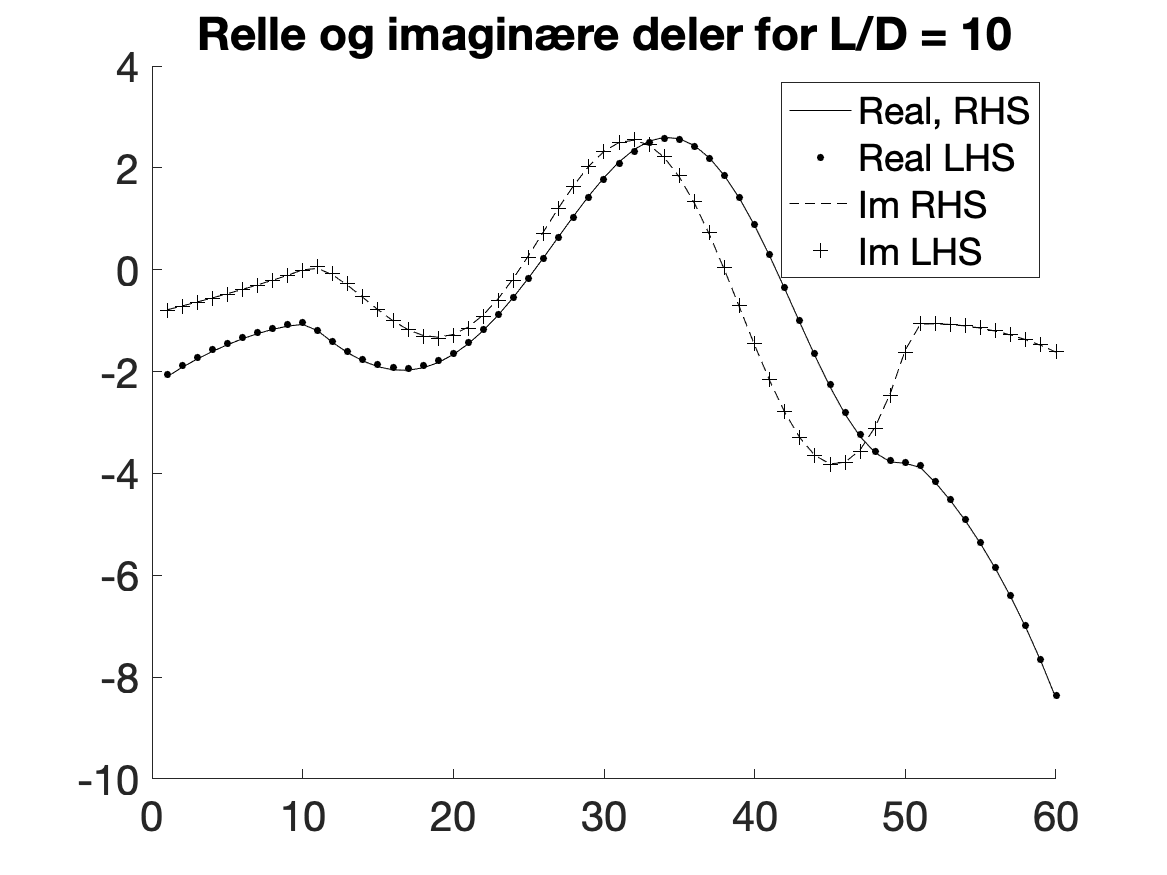
\includegraphics[width=\linewidth]{/Users/ole/Tex/MEK4420/oblig2images/plot_1_LD_1_nu09.png}
    \captionof{figure}{L/D = 10}
\end{minipage}
\hspace{0.05\linewidth}
\begin{minipage}[t]{0.45\linewidth}
    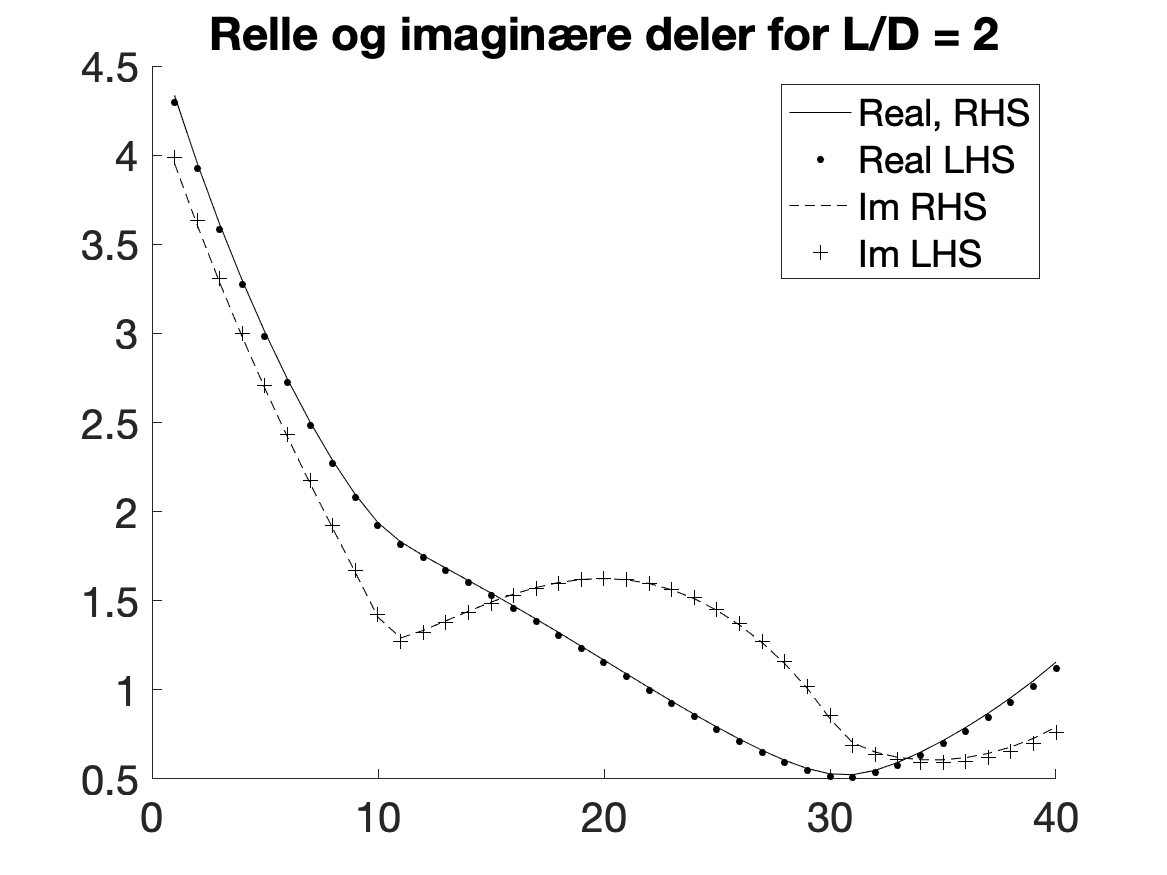
\includegraphics[width=\linewidth]{/Users/ole/Tex/MEK4420/oblig2images/plot_2_LD_2_nu09.png}
    \captionof{figure}{L/D = 2}
\end{minipage}

\vspace{0.5cm} % Adds vertical space between rows

\noindent
\begin{minipage}[t]{0.45\linewidth}
    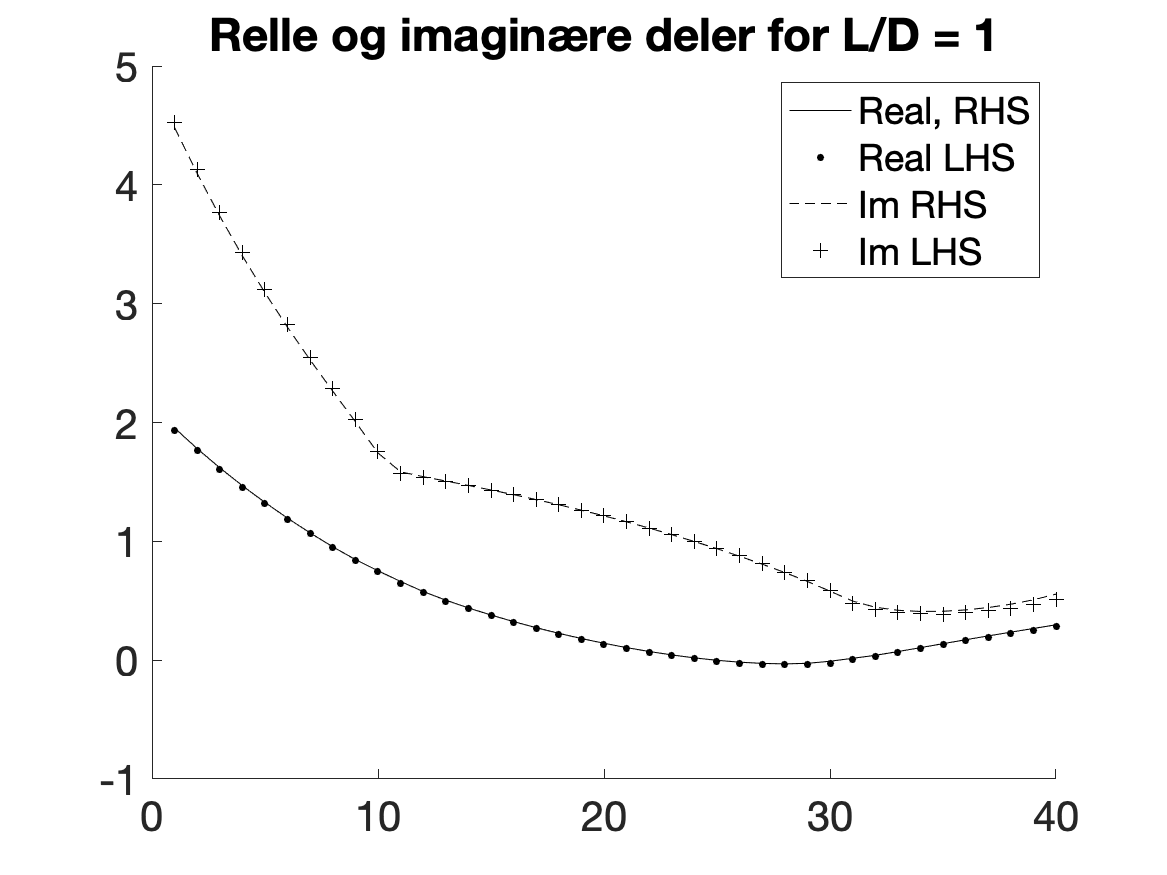
\includegraphics[width=\linewidth]{/Users/ole/Tex/MEK4420/oblig2images/plot_3_LD_3_nu09.png}
    \captionof{figure}{L/D = 1}
\end{minipage}
\hspace{0.05\linewidth}
\begin{minipage}[t]{0.45\linewidth}
    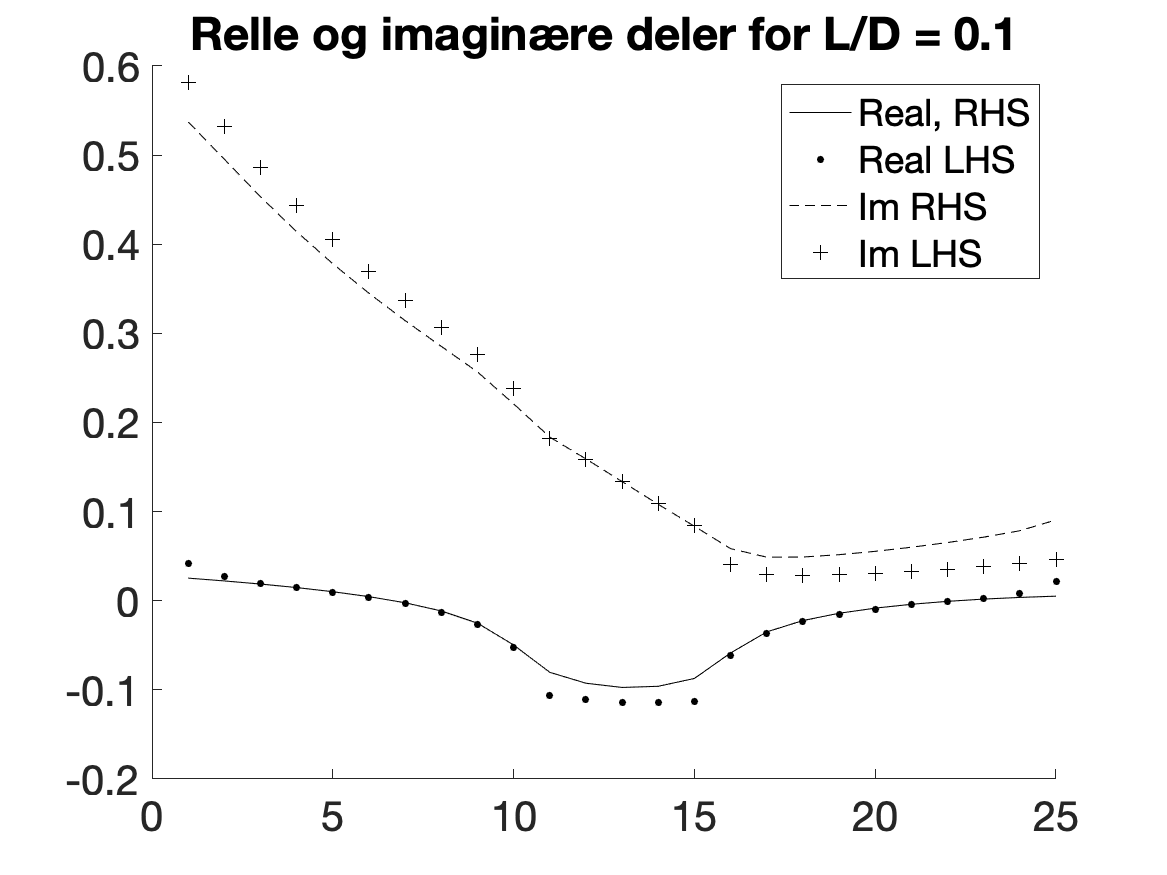
\includegraphics[width=\linewidth]{/Users/ole/Tex/MEK4420/oblig2images/plot_4_LD_4_nu09.png}
    \captionof{figure}{L/D = 0.1}
\end{minipage}

\subsection{Vi tester den numeriske løseren med KD=1.2}
\noindent
\begin{minipage}[t]{0.45\linewidth}
    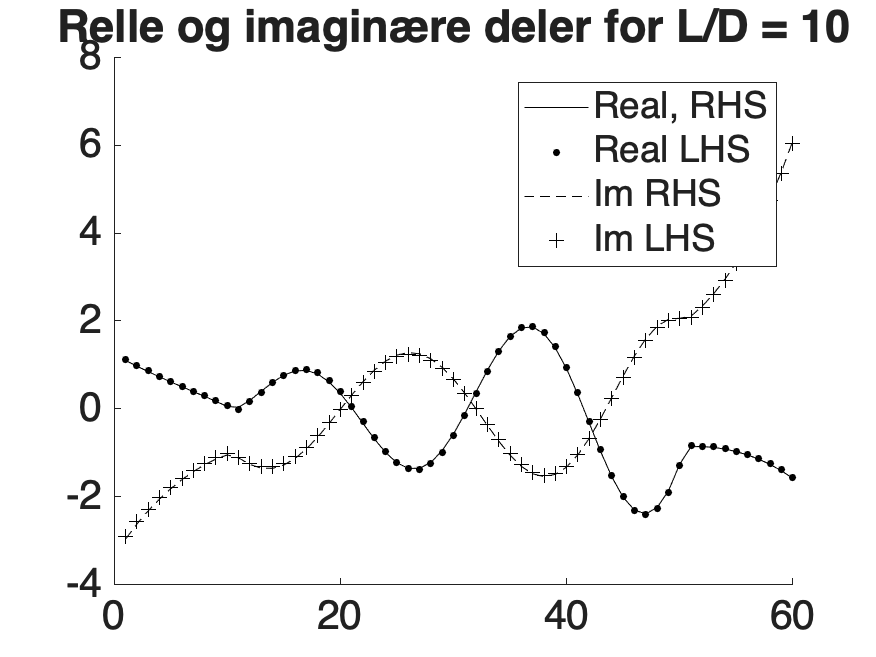
\includegraphics[width=\linewidth]{/Users/ole/Tex/MEK4420/oblig2images/plot_1_LD_1_nu12.png}
    \captionof{figure}{L/D = 10}
\end{minipage}
\hspace{0.05\linewidth}
\begin{minipage}[t]{0.45\linewidth}
    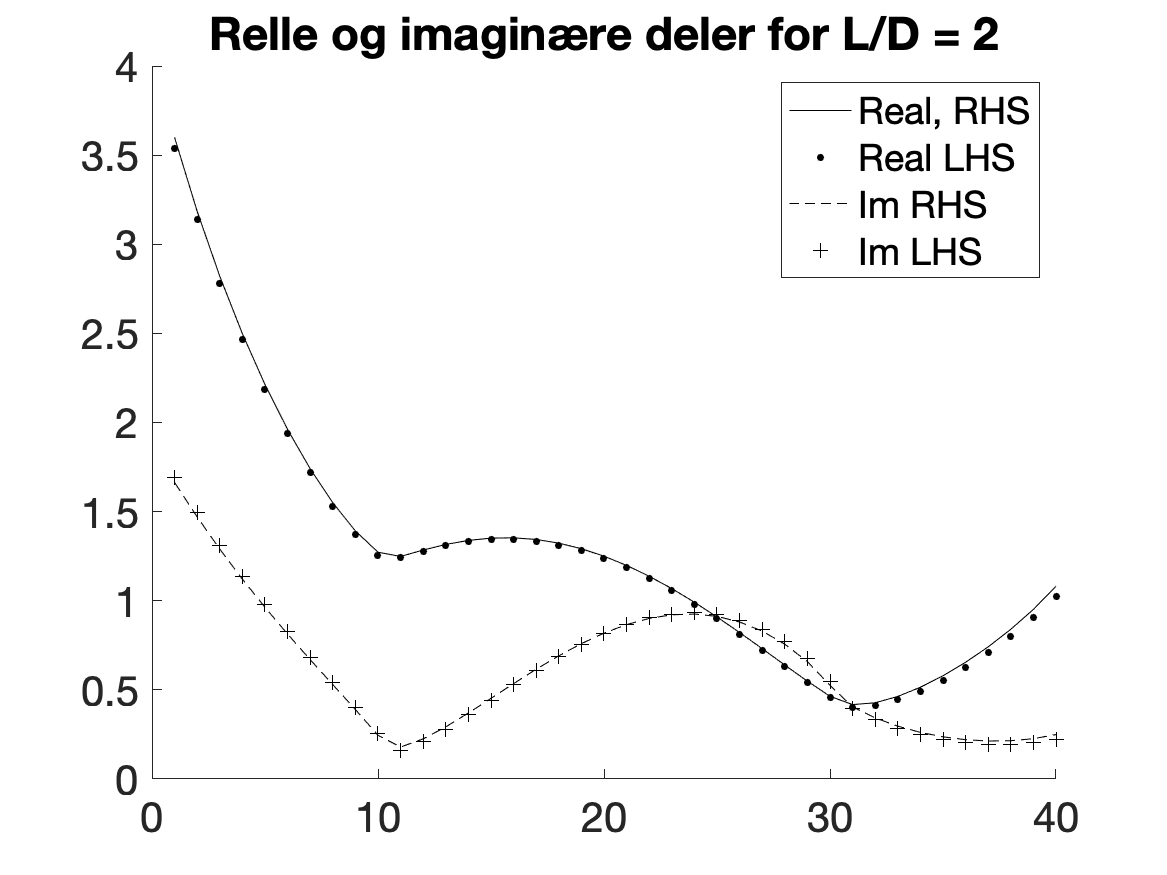
\includegraphics[width=\linewidth]{/Users/ole/Tex/MEK4420/oblig2images/plot_2_LD_2_nu12.png}
    \captionof{figure}{L/D = 2}
\end{minipage}

\vspace{0.5cm} % Adds vertical space between rows

\noindent
\begin{minipage}[t]{0.45\linewidth}
    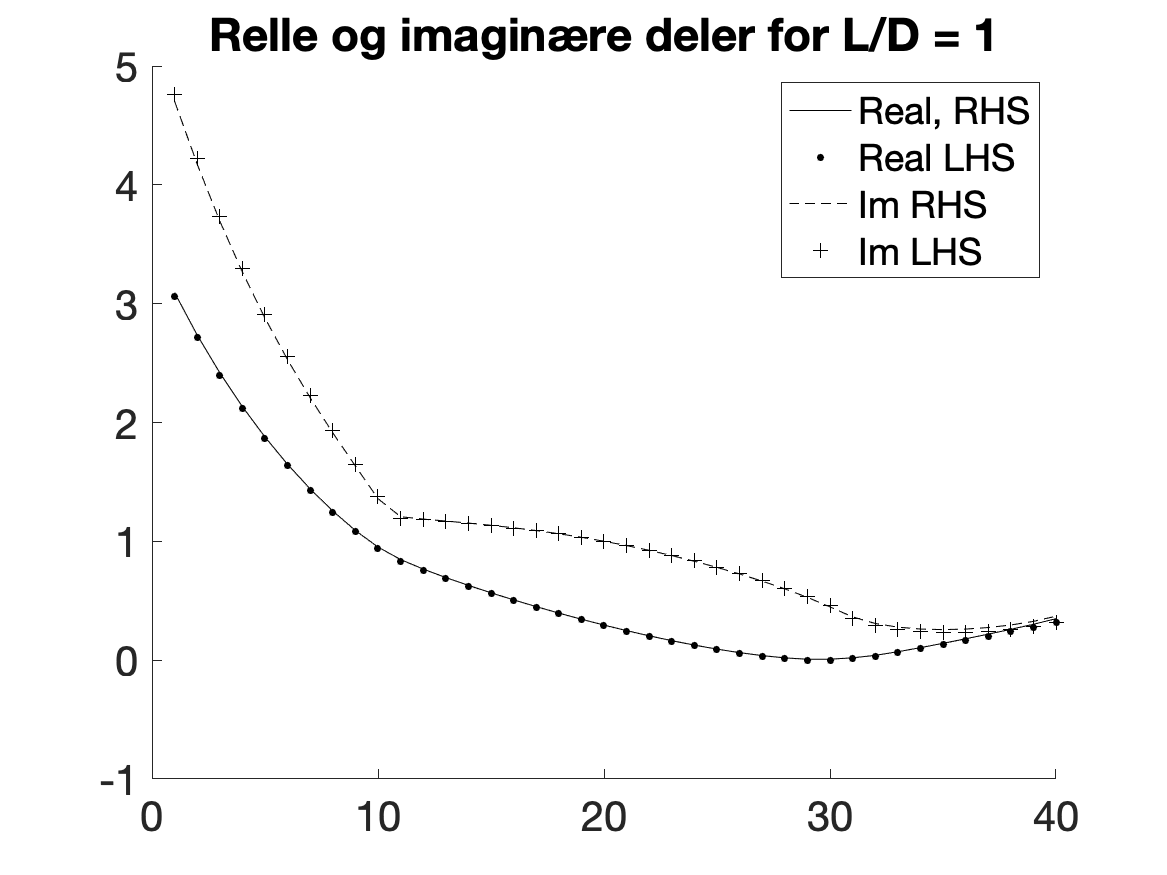
\includegraphics[width=\linewidth]{/Users/ole/Tex/MEK4420/oblig2images/plot_3_LD_3_nu12.png}
    \captionof{figure}{L/D = 1}
\end{minipage}
\hspace{0.05\linewidth}
\begin{minipage}[t]{0.45\linewidth}
    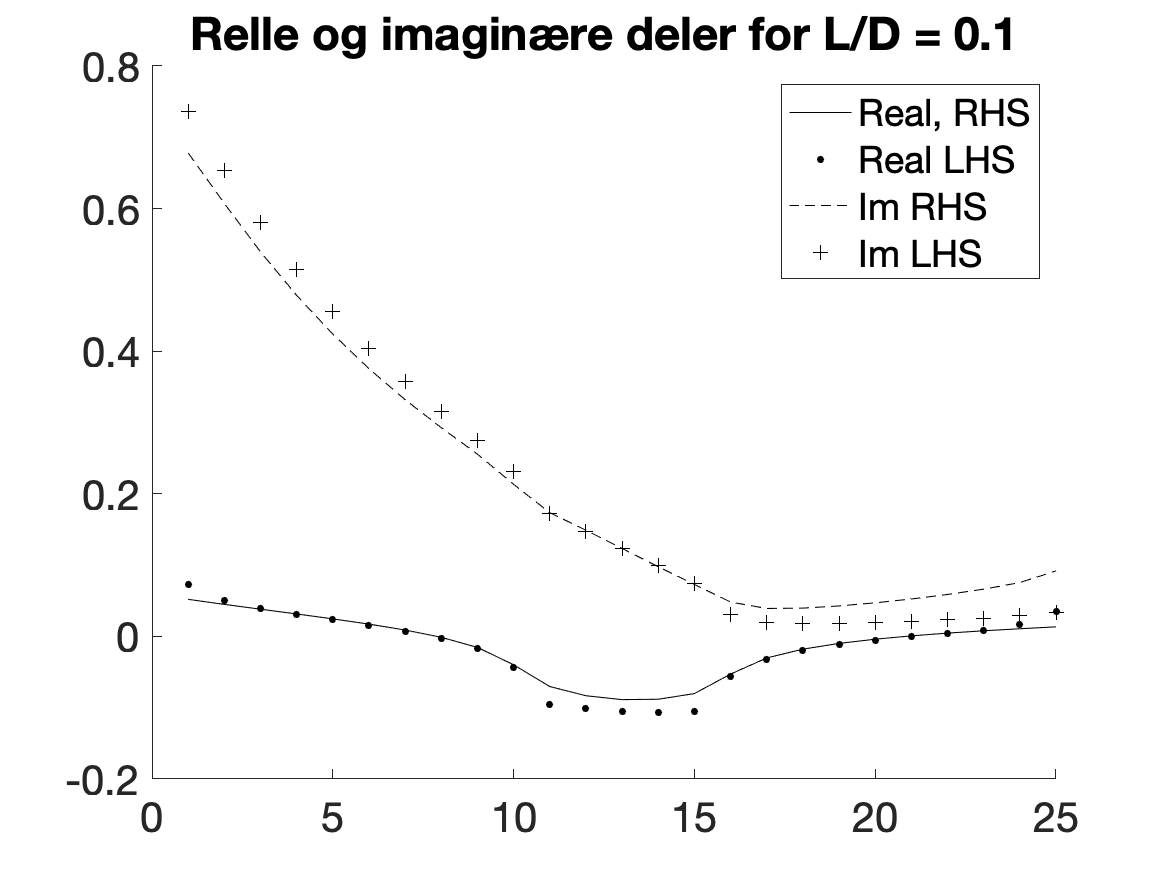
\includegraphics[width=\linewidth]{/Users/ole/Tex/MEK4420/oblig2images/plot_4_LD_4_nu12.png}
    \captionof{figure}{L/D = 0.1}
\end{minipage}


